% Young diagram of a nilpotent operator with Jordan blocks of sizes 4, 2, 2, 1.
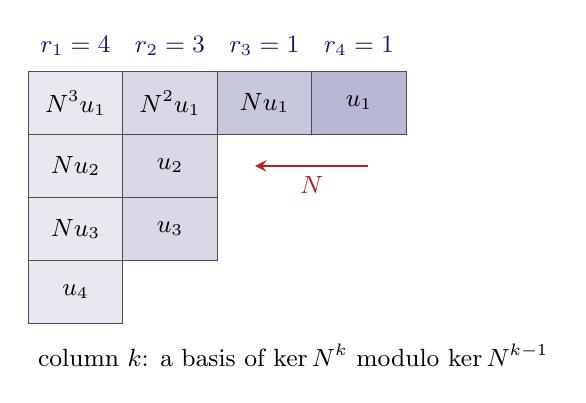
\begin{tikzpicture}[scale=0.8,>=stealth]
\filldraw[fill=MidnightBlue!10,draw=black!70] (0,0) rectangle ++(1.5,-1);
\node[font=\small] at (0.75,-0.5) {$N^{3}u_1$};
\filldraw[fill=MidnightBlue!17,draw=black!70] (1.5,0) rectangle ++(1.5,-1);
\node[font=\small] at (2.25,-0.5) {$N^{2}u_1$};
\filldraw[fill=MidnightBlue!24,draw=black!70] (3,0) rectangle ++(1.5,-1);
\node[font=\small] at (3.75,-0.5) {$Nu_1$};
\filldraw[fill=MidnightBlue!31,draw=black!70] (4.5,0) rectangle ++(1.5,-1);
\node[font=\small] at (5.25,-0.5) {$u_1$};
\filldraw[fill=MidnightBlue!10,draw=black!70] (0,-1) rectangle ++(1.5,-1);
\node[font=\small] at (0.75,-1.5) {$Nu_2$};
\filldraw[fill=MidnightBlue!17,draw=black!70] (1.5,-1) rectangle ++(1.5,-1);
\node[font=\small] at (2.25,-1.5) {$u_2$};
\filldraw[fill=MidnightBlue!10,draw=black!70] (0,-2) rectangle ++(1.5,-1);
\node[font=\small] at (0.75,-2.5) {$Nu_3$};
\filldraw[fill=MidnightBlue!17,draw=black!70] (1.5,-2) rectangle ++(1.5,-1);
\node[font=\small] at (2.25,-2.5) {$u_3$};
\filldraw[fill=MidnightBlue!10,draw=black!70] (0,-3) rectangle ++(1.5,-1);
\node[font=\small] at (0.75,-3.5) {$u_4$};
\node[font=\small,MidnightBlue] at (0.75,0.4) {$r_1=4$};
\node[font=\small,MidnightBlue] at (2.25,0.4) {$r_2=3$};
\node[font=\small,MidnightBlue] at (3.75,0.4) {$r_3=1$};
\node[font=\small,MidnightBlue] at (5.25,0.4) {$r_4=1$};
\draw[->,BrickRed,thick] (5.4,-1.5) -- (3.6,-1.5) node[midway,below,font=\small] {$N$};
\node[font=\small,anchor=west] at (0,-4.5) {column $k$: a basis of $\ker N^k$ modulo $\ker N^{k-1}$};
\end{tikzpicture}
